\section{Metod}
Först undersöktes de strukturella förbättringarna som har föreslagits i biblioteket och sedan de algoritmiska.
\subsection{Strukturella förbättringar}
Tidigare så föreslogs att matrisernas L och U matriser kunde sparas i matrix-structen så dessa inte behövdes beräknas varje gång. Detta fungerar bra så länge matrisen inte ändras och då detta behövs då kollas i alla funktioner som ändrar på matrisens innehåll. Så structen skulle isåfall innehålla två extra matriser och en booleank variabel som höll koll på om matrisen ändrades. Att testa i alla funktioner bestämdes till att vara väldigt överflödigt och om någon lägger till en funktion och glömmer lägga in testet så faller hela konceptet. Samma sak gäller om någon väljer att manipulera datan i matrisen direkt utan att använda bibliotekets funktioner så detta alternativ gick bort.

\subsection{Algoritmiska förbättringar}
Den förbättringen som valdes till den bästa för biblioteket var att använda strassen istället för den naiva algoritmen när man utförde matrismultiplikationer. Först så implementerades algoritmen och sedan så gjordes tester för att bestämma när det blev mer optimerat att använda den istället för den naiva. I den nuvarande implementation så används funktionen multiply\_matrices som innehåller den naiva algoritmen. Detta gjordes om så att den funktionen kallar på multiply\_matrices\_naive om storleken på den resulterande matrisen understiger gränsvärdet som mättes upp , annars kallar funktionen på strassen\_matrices för matrismultiplikation. 
\\
\\
För att sedan testa om biblioteket kunde utnyttja en paralleliserad version av Strassen så implementerades  strassen\_matrices\_parallel. Dock för att bibehålla kompabiliteten med alla platformen så kan all denna kod tas bort av preprocessorn genom att inte sätta PARALLEL flaggen i matLib.h
\subsection{Implementation av Strassen algoritmen}
Implementationen använder algoritmen beskriven i \ref{sec:strassen}. Dock beroende på utformning av bibliotektet så måste en ny matris skapas för varje operation man gör. Detta leder till att under en multiplikation utan rekursivt anrop så skapas och frigörs 38 matriser. 

\subsection{Jämförelser mellan algoritmer}
I figur~\ref{fig:comparison} kan man se jämförelsen mellan Strassen och naive. Upplösningen mellan punkter är rätt dålig men det tar lång tid att beräkna punkter över 500 element. Datan är dock genomsnittet av 5 tester per algoritm. Man kan tydligt se att över 500 element så har Strassen ett stort övertag över naive. 

\begin{figure}[H]
	\begin{center}
		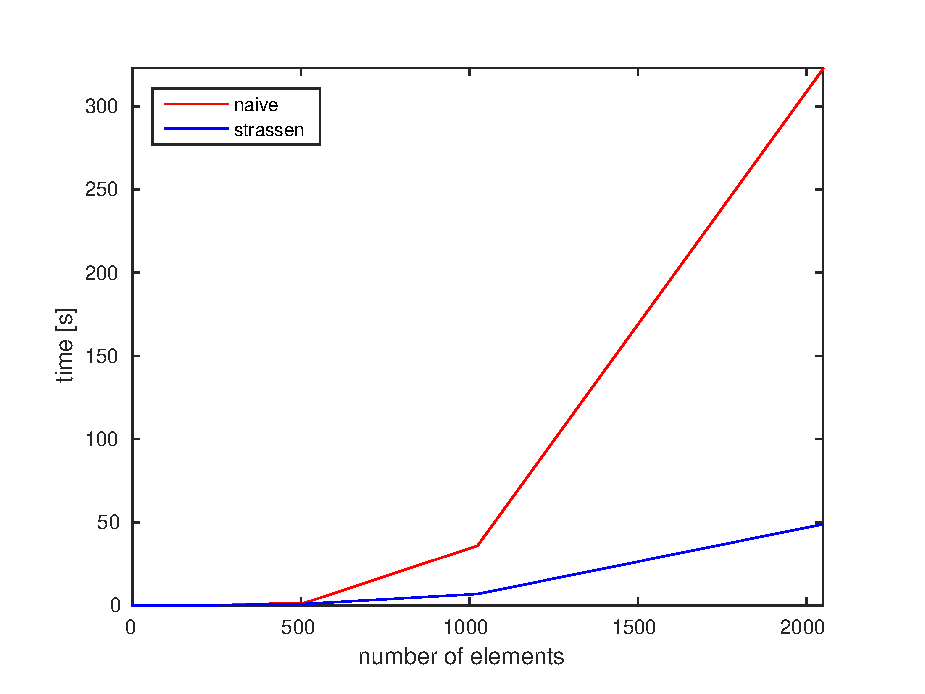
\includegraphics[scale=0.6]{martin-tex/comparison.eps}
	\end{center}
	\caption{Jämförelse mellan naive och Strassen.}
	\label{fig:comparison}
\end{figure}

\subsection{Implementation av Strassen paralelliserad}
Implementation använder algoritmen beskriven i \ref{sec:strassen}. Dock så skapas i varje rekursivt anrop sju trådar som vardera utför beräkningen av $M_{1-7}$. Den finns en global räknare som är skyddad med en semaphore som alla trådar har tillgång till. I matLib.h kan man sätta variabel number\_of\_cores till så många trådar som man vill använda. När en tråd kommer till en situation där det finns möjlighet att starta fler trådar så jämförs den globala räknaren med number\_of\_cores för att se om det finns en ledig plats. Finns det inte så utförs beräkningen med vanliga strassen\_matrices. 


